% 1960 年全国卷第 9 题：y=-x^2+3x 的图象。
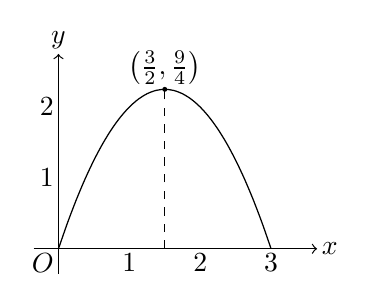
\begin{tikzpicture}[scale=0.9, line width=0.45pt,
  every node/.style={inner sep=1.5pt}]
  \draw[->] (-0.35,0)--(3.65,0) node[anchor=west] {$x$};
  \draw[->] (0,-0.35)--(0,2.75) node[anchor=south] {$y$};
  \draw[dashed] (1.5,0)--(1.5,2.25);
  \draw[domain=0:3,smooth,variable=\x] plot (\x,{-(\x)^2+3*\x});
  \fill (1.5,2.25) circle (0.035);
  \node[anchor=north east] at (0,0) {$O$};
  \node[anchor=north] at (1,0) {$1$};
  \node[anchor=north] at (2,0) {$2$};
  \node[anchor=north] at (3,0) {$3$};
  \node[anchor=east] at (0,1) {$1$};
  \node[anchor=east] at (0,2) {$2$};
  \node[anchor=south] at (1.5,2.25) {$\left(\frac32,\frac94\right)$};
\end{tikzpicture}
